\newpage
\thispagestyle{empty}
\section{Контрольная работа 4}


\subsection[2018-2019]{\hyperref[sec:sol_kr_04_2018_2019]{2018-2019}}
\label{sec:kr_04_2018_2019}

Комментарий: минимум писали 30 минут без официальных шпаргалок, основную часть 90 минут — с листом А4. 

\subsubsection*{Минимум}


\begin{enumerate}

%Задача №1
\item Пусть $X_{1}, \ldots, X_{n}$ — случайная выборка из нормального распределения с неизвестным математическим ожиданием $\mu$ и известной дисперсией $\sigma^2=100$. Объем выборки $n=25$. Для тестирования основной гипотезы $H_{0}:\mu=(-1)$ против альтернативы $H_{1}:\mu=0$ Винни-Пух использует простой критерий. Если $\bar X \leq (-0.5)$, то Винни-Пух не отвергает гипотезу $H_{0}$, в противном случае Винни-Пух отвергает гипотезу $H_{0}$ в пользу гипотезы $H_{1}$. 

Найдите:

\begin{enumerate}
    \item вероятность ошибки 1-го рода;
    \item вероятность ошибки 2-го рода;
    \item мощность критерия.
\end{enumerate}

%Задача №2
\item Пусть $X_{1}, \ldots, X_{n}$ — случайная выборка из нормального распределения $\cN(\mu, \sigma^2)$ с неизвестными параметрами $\mu$ и ${\sigma}^2$.
Используя реализацию случайной выборки,
\[
x_{1} = -2, \quad x_{2} = -1, \quad x_{3} = 0, \quad x_{4} = 1, \quad x_{5} = 2
\]
постройте 90\%-ый доверительный интервал для неизвестного параметра $\sigma^2$.

%Задача №3
\item Пусть $X_{1}, \ldots, X_{n}$ и $Y_{1}, \ldots, Y_{m}$ — независимые случайные
выборки из нормальных распределений $\cN(\mu_{X},\sigma^2_{X})$ и
$\cN(\mu_{Y},\sigma^2_{Y})$ соответственно.
Уровень значимости $\alpha = 0.1$.

Используя реализации случайных выборок

\begin{align*}
x_{1} &= -2, \quad x_{2} = -1, \quad x_{3} = 0, \quad x_{4} = 1, \quad x_{5} = 2, \\
y_{1} &= -2, \quad y_{2} = 0, \quad y_{3} = 2,
\end{align*}
проверьте гипотезу о равенстве дисперсий $\sigma^2_X = \sigma^2_Y$ против гипотезы о неравенстве дисперсий.

%Задача №4
\item Пусть $X_{1}, \ldots, X_{n}$ и $Y_{1}, \ldots, Y_{m}$ —
независимые случайные выборки из нормальных распределений 
$\cN(\mu_{X},\sigma^2)$ и $\cN(\mu_{Y},\sigma^2)$ соответственно.

Используя реализации случайных выборок
\begin{align*}
x_{1} &= -2, \quad x_{2} = -1, \quad x_{3} = 0, \quad x_{4} = 1, \quad x_{5} = 2, \\
y_{1} &= -2, \quad y_{2} = 0, \quad y_{3} = 2,
\end{align*}
постройте 60\%-ый доверительный интервал для разности математических ожиданий
$\mu_{X} - \mu_{Y}$.

%Задача 5
\item Пусть $X_{1}, \ldots, X_{n}$ и $Y_{1}, \ldots, Y_{m}$ — две независимые случайные выборки из распределения Бернулли с неизвестными параметрами $p_{X}\in(0,1)$ и $p_{Y}\in(0,1)$. Известно, что $n=100$, $m=150$, $\sum_{i=1}^{n}x_{i}=60$, $\sum_{i=1}^{n}y_{i}=50$. На уровне значимости $\alpha=0.05$ протестируйте гипотезу $H_{0}:p_{X}=p_{Y}$ против альтернативной гипотезы $H_{1}:p_{X}>p_{Y}$.


\end{enumerate}

\subsubsection*{Основная часть}


\begin{enumerate}

%Задача №1

\item Пусть $X$ — случайная выборка, содержащая одно наблюдение, из распределения с функцией плотности

\[
f_X(x) =
	\begin{cases}
	\theta x^{\theta-1},\text{ при }  x \in [0; 1] \\
	0\quad \quad \text{, }\text{ при } x \notin  [0; 1] \\
	\end{cases},
\]

где $\theta>0$ — неизвестный параметр распределения. Тестируется основная гипотеза $H_{0}:\theta=1$ против альтернативной гипотезы $H_{1}:\theta=2$.

\begin{enumerate}
    \item (7) С помощью леммы Неймана–Пирсона найдите наиболее мощный критерий, имеющий уровень значимости $\alpha=0.05$.
    \item (3) Вычислите мощность полученного критерия.
\end{enumerate}

%Задача №2

\item На раскопках старинного замка Вася нашел древнюю монетку. Монетка ему показалась крайне необычной, и поэтому он решил провести серию из 100 подбрасываний. Результаты Вася записал в таблицу.

\begin{center}\begin{tabular}{rrrr}
\toprule
   & Орел   & Решка & Ребро  \\ \midrule
Количество раз &   $40$ & $50$ & $10$ \\ \bottomrule
\end{tabular}\end{center}
\begin{enumerate}
    \item (6) Постройте двусторонний 95\%-ый доверительный интервал для вероятности выпадения ребра.
    \item (4) На уровне значимости 5\% проверьте гипотезу о том, что ребро выпадает в одном случае из 100 против альтернативы, что чаще, и вычислите соответствующее $P$-значение.
    \item (10) С помощью теста отношения правдоподобия на уровне значимости 10\% проверьте гипотезу о том, что орёл выпадает так же часто, как решка, и в три раза чаще, чем ребро.
    \item (5) С помощью критерия согласия Пирсона на уровне значимости 10\% проверьте гипотезу из предыдущего пункта.
\end{enumerate}

Подсказка: $\ln 2 \approx 0.7$, $\ln 3 \approx 1.1$, $\ln 5 \approx 1.6$, $\ln 7 \approx 1.95$, $\ln 11 \approx 2.4$.

%Задача №3

\item Губка Боб и Патрик ловят медуз для коллекции. Число пойманных за $i$-ый день медуз имеет распределение Пуассона с неизвестным параметром $\lambda$. Уловы медуз в различные дни независимы. За прошедшие $100$ дней они поймали $300$ медуз. 

\begin{enumerate}
    \item (5) С помощью асимптотических свойств оценок максимального правдоподобия постройте 95\%-ый доверительный интервал для неизвестного параметра $\lambda$.
    \item (10) С помощью дельта-метода постройте приближенную 95\%-ую интервальную оценку вероятности того, что за 101-ый день Губка Боб и Патрик не поймают ни одной медузы.
\end{enumerate}

\end{enumerate}





\subsection[2017-2018]{\hyperref[sec:sol_kr_04_2017_2018]{2017-2018}}
\label{sec:kr_04_2017_2018}


\subsubsection*{Минимум}

\begin{enumerate}


	\item Пусть $X=(X_{1}, \ldots,X_{n})$ — случайная выборка из нормального распределения с неизвестным математическим ожиданием $\mu$ и неизвестной дисперсией $\sigma^2=9$. Объем выборки $n=20$. Для тестирования основной гипотезы $H_{0}:\mu=0$ против альтернативной гипотезы $H_{1}:\mu=5$ вы используете критерий: если $\overline{X}\leq2$, то вы не отвергаете гипотезу $H_{0}$, в противном случае вы отвергаете гипотезу $H_{0}$ в пользу гипотезы $H_{1}$. Найдите
	\begin{enumerate}
	\item Вероятность ошибки 1-го рода
	\item Вероятносто ошибки 2-го рода
	\end{enumerate}


		\item Пусть $X=(X_{1}, \ldots,X_{n})$ — случайная выборка из нормального распределения с неизвестными параметрами $\mu$ и $\sigma^2$. Используя реализацию случайной выборки: $x_{1}=2$, $x_{3}=8$, $x_{3}=5$, постройте 95\%-ый доверительный интервал для неизвестного параметра $\sigma^2$.


	\item Вася очень любит тестировать статистические гипотезы. В этот раз Вася собирается проверить утверждение о том, что его друг Пётр звонит Васе исключительно в то время, когда Вася ест. Для этого Вася трудится целый год и проводит серию из 365 испытаний. Результаты приведены в табилце ниже.

	\begin{center}
		\begin{tabular}{c|cc}
			\toprule
			& Пётр не звонит & Пётр звонит\\
			\midrule
			Вася ест & $100$ & $50$\\
			Вася не ест  & $125$ & $90$\\
			\bottomrule
		\end{tabular}
	\end{center}

	На уровне значимости 10\% протестируйте гипотезу о том, что Пётр звонит Васе независимо от момента приема пищи.


\item Вася Сидоров утверждает, что ходит в кино в четыре раза чаще, чем в спортзал, а в спортзал в четыре раза чаще, чем в театр.
За последние полгода он 105 раз был в театре, 63 раза — в спортазе и 42 раза в кино.
На уровне значимости 10\% проверьте утверждение Васи.

\end{enumerate}


	\begin{center}
	Квантили $\chi^2$ распределения c 1, 2 и 3 степенями свободы\\
		\begin{tabular}{c|cccccc}
			\toprule
			& 0.025 & 0.05 & 0.1 & 0.9 & 0.95 & 0.975\\
			\midrule
							1 & 0.001 & 0.004 & 0.016 & 2.706 & 3.841 & 5.024 \\
							2 & 0.051 & 0.103 & 0.211 & 4.605 & 5.991 & 7.378 \\
							3 & 0.216 & 0.352 & 0.584 & 6.251 & 7.815 & 9.348 \\
			\bottomrule
		\end{tabular}
	\end{center}

\newpage

\subsubsection*{Задачи}

При решении задач пять–семь используйте данные обследования Росстата за первый квартал 2018 года:

	\begin{center}
		\begin{tabular}{c|ccc}
			\toprule
			& Число наблюдений & Среднее (тыс. руб.) & Выборочное отклонение (тыс. руб.) \\
			\midrule
							Врачи & 40 & 136 & 55  \\
							Преподаватели & 60 & 139 & 60 \\
			\bottomrule
		\end{tabular}
	\end{center}

Распределение заработной платы работников любой отрасли хорошо описывается нормальным законом.

\begin{enumerate}[resume]

	%Задача 1
	\item На уровне значимости 5\% проверьте гипотезу о том, что средняя зарплата врача составляет 100 т.р., против альтернативы, что она больше 100 т.р.  Вычислите минимальный уровень значимости, при котором основная гипотеза отвергается (Р–значение).

	%Задача 2
	\item На уровне значимости 10\% проверьте гипотезу о том, что разброс в зарплатах врачей и преподавателей одинаков, против двухсторонней альтернативы.

	%Задача 3
	\item На уровне значимости 10\% проверьте гипотезу о том, что средняя зарплата врачей и преподавателей совпадают, против альтернативы, что у преподавателей зарплата выше:

	\begin{enumerate}
	\item Считая объемы выборок достаточно большими
			\item Считая дисперсии одинаковыми
	 \end{enumerate}

			%Задача 4
			\item Время в часах безотказной работы  микронаушника, величина $X$, подчиняется экспоненциальному (показательному) закону распределения с неизвестным параметром $\lambda$:
\[
f(x;\lambda)
			=\begin{cases}
			\lambda e^{-\lambda x},\text{ при } x\geq0\\
			0, \text{ при }  x<0\\
			\end{cases}
\]
По выборке из 100 независимых наблюдений $\bar x=0.52$. С помощью асимптотических свойств оценок максимального правдоподобия постройте приближенный 95\%-ый доверительный интервал:

\begin{enumerate}
	\item Для параметра $\lambda$
			\item Для вероятности того, что наушник проработает без сбоев весь тест — 45 минут
	 \end{enumerate}

	 %Задача 5
	 \item Приглашенный на Петербургский международный экономический форум Германом Грефом индийский мистик Садхгуру подарил Грефу древнюю шестигранную кость для принятия решений в сложных макроэкономических ситуациях. Служба безопасности Сбербанка провела серию из 100 испытаний и составила таблицу:

			 \begin{center}
		\begin{tabular}{c|cccccc}
			\toprule
			Грань & 1 & 2 & 3 & 4 & 5 & 6\\
			\midrule
							Число выпадений & 10 & 10 & 15 & 15 & 25 & 25 \\
			\bottomrule
		\end{tabular}
	\end{center}

С помощью теста отношения правдоподобия на уровне значимости 5\% проверьте гипотезу о том, что все грани равновероятны.

\[
\ln(1/6)=-1.79, \; \ln(0.15)=-1.90, \; \ln(0.25)=-1.39, \; \ln(0.1)=-2.30
\]

\end{enumerate}


\newpage
\subsection[2016-2017]{\hyperref[sec:sol_kr_04_2016_2017]{2016-2017}}
\label{sec:kr_04_2016_2017}


\subsubsection*{I. Теоретический минимум}


В пунктах 1, 3, 11 и 12 предполагается, что $X = (X_1, \, \ldots, \, X_n)$ и
$Y = (Y_1, \, \ldots, \, Y_m)$ — две независимые случайные выборки из нормальных
распределений $N(\mu_X, \sigma_X^2)$ и $N(\mu_Y, \sigma_Y^2)$ соответственно.

\begin{enumerate}
  \item Приведите формулу статистики, при помощи которой можно проверить гипотезу
	$H_0 \colon \sigma_X^2 = \sigma_Y^2$. Укажите распределение этой статистики при
	верной гипотезе $H_0$.
  \item Приведите формулу информации Фишера о параметре $\theta$, содержащейся в
	одном наблюдении случайной выборки.
  \item Приведите формулу статистики, при помощи которой можно проверить гипотезу
	$H_0 \colon \mu_X - \mu_Y = \Delta_0$ при условии, что дисперсии $\sigma_X^2$
	и $\sigma_Y^2$ неизвестны, но равны между собой. Укажите распределение этой
	статистики при верной гипотезе $H_0$.
  \item Дайте определение критической области.
  \item Приведите формулу плотности нормального распределения $\cN(\mu, \sigma^2)$.
  \item Приведите формулы границ доверительного интервала с уровнем доверия
	$(1 - \alpha)$, $\alpha \in (0;\,1)$, для вероятности появления успеха в
	случайной выборке $X = (X_1, \, \ldots, \, X_n)$ из распределения Бернулли с
	параметром $p \in (0;\,1)$.
  \item Дайте определение несмещенной оценки $\hat{\theta}$ для неизвестного
	параметра $\theta \in \Theta$.
  \item Дайте определение эффективной оценки $\hat{\theta}$ для неизвестного
	параметра $\theta \in \Theta$.
  \item Приведите формулу выборочной дисперсии.
  \item Приведите формулу выборочной функции распределения.
  \item Приведите формулы границ доверительного интервала с уровнем доверия
	$(1 - \alpha)$, $\alpha \in (0;\,1)$, для $\mu_X$ при условии, что дисперсия
	$\sigma_X^2$ известна.
  \item Укажите распределение статистики $\frac{\overline{X} - \mu_X}{\sigma / \sqrt{n}}$.
\end{enumerate}


\subsubsection*{II. Задачи}

\begin{enumerate}
\item В ходе анкетирования ста сотрудников банка «Альфа» были получены ответы на
вопрос о том, сколько времени они проводят на работе ежедневно. Среднее выборочное
оказалось равным $9.5$ часам, а выборочное стандартное отклонение $0.5$ часа.
\begin{enumerate}
  \item На уровне значимости 5\,\% проверьте гипотезу о том, что сотрудники банка
	«Альфа» в среднем проводят на работе $10$ часов, против альтернативной гипотезы о
	том, что сотрудники банка «Альфа» в среднем проводят на работе менее $10$ часов.
  \item Найдите точное $P$-значение для наблюдаемой статистики из пункта (a).
  \item Сформулируйте предпосылки, которые были использованы вами для выполнения
	пункта (a).
  \item На уровне значимости 5\,\% проверьте гипотезу о $H_0 \colon \sigma^2 = 0.3$.
\end{enumerate}


\item Проверка сорока случайно выбранных лекций показала, что студент Халявин
присутствовал только на 16 из них. На уровне значимости 5\,\% проверьте гипотезу
о том, что Халявин посещает в среднем половину лекций.

\item В ходе анкетирования двадцати сотрудников банка «Альфа» были получены ответы
на вопрос о том, сколько времени они проводят на работе ежедневно. Среднее выборочное
оказалось равным $9.5$ часам, а выборочное стандартное отклонение $0.5$ часа.
Аналогичные показатели для 25 сотрудников банка «Бета» составили $9.8$ и $0.6$
часа соответственно.
\begin{enumerate}
  \item На уровне значимости 5\,\% проверьте гипотезу о равенстве математических
	ожиданий времени, проводимого на работе сотрудниками банков «Альфа» и «Бета».
  \item Сформулируйте предпосылки, которые были использованы вами для выполнения
	пункта (a).
  \item На уровне значимости 5\,\% проверьте гипотезу о равенстве дисперсий времени,
	проводимого на работе сотрудниками банков «Альфа» и «Бета».
\end{enumerate}

\item Вася решил проверить известное утверждение о том, что бутерброд падает
маслом вниз. Для этого он провел серию из 200 испытаний. Ниже приведена таблица
с результатами:
\begin{center}
\begin{tabular}{ccc}
  \toprule
  \text{Бутерброд}                &\text{Маслом вниз}    &\text{Маслом вверх}       \\ \midrule
  \text{Число наблюдений}         &$105$    &$95$       \\ \bottomrule
\end{tabular}
\end{center}
Можно ли утверждать, что бутерброд падает маслом вниз так же часто, как и маслом
вверх? При ответе на вопрос используйте уровень значимости 5\,\%.

\item Пусть $X = (X_1, \, \ldots, \, X_{100})$ — случайная выборка из нормального
распределения с математическим ожиданием $\mu$ и дисперсией $\nu$. Оба параметра
$\mu$ и $\nu$ неизвестны. Используя следующие данные $\sum_{i=1}^{100}x_i = 30$,
$\sum_{i=1}^{100}x_i^2 = 146$ и $\sum_{i=1}^{100}x_i^3 = 122$ с помощью теста
отношения правдоподобия проверьте гипотезу $H_0 \colon \nu = 1$ на уровне значимости 5\,\%.
\end{enumerate}


\newpage
\subsection[2015-2016]{\hyperref[sec:sol_kr_04_2015_2016]{2015-2016}}
\label{sec:kr_04_2015_2016}

\begin{enumerate}
\item	Сформулируйте определения несмещённости, состоятельности и эффективности оценок.
\item На курсе учится 250 человек. Предположим, что число студентов, не явившихся
на экзамен, хорошо описывается законом Пуассона.
\begin{enumerate}
\item	Методом максимального правдоподобия найдите оценку параметра распределения Пуассона.
\item	Проверьте выполнение свойств несмещенности, эффективности и состоятельности
для данной оценки.
\item	Найдите оценку максимального правдоподобия для вероятности стопроцентной
явки студентов на экзамен.
\item	Используя дельта-метод, постройте для этой вероятности асимптотический
доверительный интервал.
\end{enumerate}

\item	Фармацевтическая компания выпустила новое лекарство от бессонницы, утверждая,
что оно помогает 80\% людей, страдающих бессонницей. Чтобы проверить утверждение
компании, случайным образом выбираются 20 человек, страдающих бессонницей. Обозначим
за $Y$ количество человек из выборки, которым лекарство помогло. Основная гипотеза,
$H_0$: $p=0.8$, альтернативная гипотеза $H_a$: $p=0.6$. Критическая область: $\{Y<12\}$.
\begin{enumerate}
\item	В терминах этой задачи сформулируйте, что является ошибкой первого рода.
Найдите уровень значимости, соответствующий заданной критической области.
\item	В терминах этой задачи сформулируйте, что является ошибкой второго рода.
Найдите вероятность ошибки второго рода.
\item	Найдите такое значение $c$, что вероятность ошибки первого рода $\alpha
\approx 0.1$ при критической области вида $\{Y<c\}$. Найдите соответствующее
значение вероятности ошибки второго рода.
\item	Каким должен быть размер выборки, чтобы выборочная доля страдающих бессонницей
отличалась от истинной вероятности не более, чем на $0.01$ с вероятностью не менее,
чем $0.95$?
\end{enumerate}

\item	Вася Сидоров утверждает, что ходит в кино в два раза чаще, чем на лекции
по статистике, на лекции по статистике в два раза чаще, чем в спортзал. За
последние полгода он 10 раз был в спортзале, 1 раз — на лекциях по статистике и
39 раз в кино.

При помощи критерия хи-квадрат Пирсона на уровне значимости $0.05$ проверьте,
правдоподобно ли Васино утверждение.

\item У Евдокла есть случайная выборка из экспоненциального распределения с
неизвестным параметром $\lambda$ в 50 наблюдений, $X_1$, $X_2$, \ldots, $X_{50}$.
Оказалось, что $\bar X = 1.1$. Евдокл хочет проверить гипотезу о равенстве
$\lambda = 1$ против альтернативной гипотезы о неравенстве $\lambda \neq 1$ на
уровне значимости $0.1$.

Помогите Евдоклу и проверьте гипотезу с помощью критерия отношения правдоподобия.

Пачка логарифмов: $\ln 50 \approx 3.9$, $\ln 55 \approx 4.0$, $\ln 11 \approx 2.4$,
$\ln 60 \approx 4.1$, $\ln 12 \approx 2.5$

\item Американский демографический журнал опубликовал исследование, в котором
утверждается, что посетители крупных торговых центров за одно посещение тратят
в выходные дни больше, чем в будние. Наибольшие расходы приходятся на воскресенье
в период с 4 до 6 часов вечера. Для двух независимых выборок посетителей средние
расходы и выборочные стандартные отклонения расходов составили
\begin{center}
\begin{tabular}{lrr}
\toprule
 & Выходные & Рабочие дни \\
\midrule
Число наблюдений & 21 & 19 \\
Средние расходы (\$) & 78 & 67 \\
Выборочное стандартное отклонение (\$) & 22 & 20 \\
\bottomrule
\end{tabular}
\end{center}

\begin{enumerate}
\item Проверьте гипотезу о равенстве дисперсий расходов
\item Предполагая, что дисперсии расходов одинаковы, проверьте гипотезу об отсутствии
разницы в расходах в выходные и будние дни.
\item Сформулируйте все необходимые для проверки гипотез предыдущих пунктов предпосылки.
\end{enumerate}

\item Винни Пух знает, что пчёлы и мёд бывают правильные и неправильные.
По результатам 100~попыток добыть мёд Винни Пух составил таблицу сопряженности признаков.

\begin{center}
\begin{tabular}{lrr}
\toprule
 & Мёд правильный & Мёд неправильный \\
\midrule
Пчёлы правильные & 12	& 36 \\
Пчёлы неправильные & 32	& 20 \\
\bottomrule
\end{tabular}
\end{center}

На уровне значимости $0.05$ проверьте гипотезу о независимости характеристик пчёл и мёда.

\begin{figure}[b]
\centering
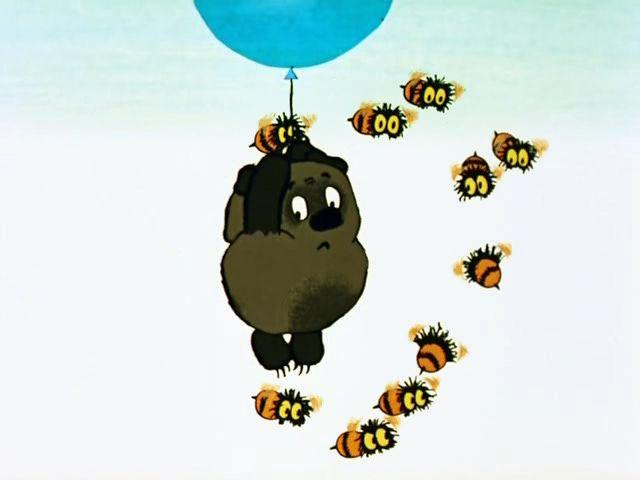
\includegraphics[width=9cm]{images/winnie_kr_4}
\end{figure}
\end{enumerate}



\newpage
\subsection[2014-2015]{\hyperref[sec:sol_kr_04_2014_2015]{2014-2015}}
\label{sec:kr_04_2014_2015}

\begin{enumerate}

\item[1.] \textbf{Задача для первого потока.}

Проверка 40 случайно выбранных лекций показала, что студент Халявин присутствовал
только на 16 из них.
\begin{enumerate}
\item Найдите 95\% доверительный интервал для вероятности увидеть Халявина на лекции.
\item На уровне значимости 5\% проверьте гипотезу о том, что Халявин посещает
в среднем половину лекций.
\item Вычислите минимальный уровень значимости, при котором основная гипотеза
отвергается (P-значение).
\end{enumerate}

\item[1.] \textbf{Задача для второго потока.}

Вес упаковки с лекарством является нормальной случайной величиной.
Взвешивание 20~упаковок показало, что выборочное среднее равно 51 г., а
несмещенная оценка дисперсии равна~4.
\begin{enumerate}
\item На уровне значимости 10\% проверьте гипотезу, что в среднем вес упаковки
составляет~55 г.
\item Контрольное взвешивание 30 упаковок такого же лекарства другого производителя
показало, что несмещенная оценка дисперсии веса равна 6. На уровне значимости 10\%
проверьте гипотезу о равенстве дисперсий веса упаковки двух производителей.
\end{enumerate}

\item[2.] \textbf{Задача для первого потока.}

В ходе анкетирования 15 сотрудников банка «Альфа» ответили на вопрос о том,
сколько времени они проводят на работе ежедневно. Среднее выборочное оказалось
равно $9.5$ часам при выборочном стандартном отклонении $0.5$ часа. Аналогичные
показатели для 12 сотрудников банка «Бета» составили $9.8$ и $0.6$ часа соответственно.

Считая распределение времени нормальным, на уровне значимости 5\% проверьте
гипотезу о том, что сотрудники банка «Альфа» в среднем проводят на работе столько
же времени, сколько и сотрудники банка «Бета».

\item[2.] \textbf{Задача для второго потока.}

Экзамен принимают два преподавателя, случайным образом выбирая студентов.
По выборке из 85 и 100 наблюдений, выборочные доли не сдавших экзамен студентов составили
соответственно $0.2$ и $0.17$.
\begin{enumerate}
\item Можно ли при уровне значимости в 1\% утверждать, что преподаватели предъявляют
к студентам одинаковый уровень требований?
\item Вычислите минимальный уровень значимости, при котором основная гипотеза
отвергается (P-значение).
\end{enumerate}

\item[3.] Методом максимального правдоподобия найдите оценку параметра $\theta$
для выборки $X_1$, \ldots, $X_n$ из распределения с функцией плотности
\[
f(x)=\begin{cases}
\frac{1}{\theta^2}xe^{-\frac{x}{\theta}}, \; x>0 \\
0, \; x\leq 0
\end{cases}
\]

\item[4.]
Пусть $X_1$, \ldots, $X_{100}$ — случайная выборка из нормального распределения
с математическим ожиданием $\mu$ и дисперсией $\nu$, где $\mu$ и $\nu$ — неизвестные
параметры. По 100 наблюдениям $\sum x_i=30$, $\sum x_i^2=146$, $\sum x_i^3=122$.

При помощи теста отношения правдоподобия протестируйте гипотезу $H_0: \nu=1$
на уровне значимости 5\%.

\item[5.] \textbf{Исследовательская задача.}

Пусть $X_1$, \ldots, $X_{n}$ — случайная выборка из нормального распределения
с математическим ожиданием $\mu$ и дисперсией $\nu$, где $\mu$ и $\nu$ — неизвестные
параметры. Рассмотрим три классических теста, отношения правдоподобия, $LR$,
множителей Лагранжа, $LM$ и Вальда, $W$, для тестирования гипотезы $H_0: \; \mu=0$.

\begin{enumerate}
\item Сравните  статистики $LR$, $LM$ и $W$ между собой. Какая — наибольшая,
какая — наименьшая?
\item Изменится ли упорядоченность статистик, если проверять гипотезу $H_0: \; \mu=\mu_0$?
\end{enumerate}

Подсказка: $\frac{x}{1+x} \leq \ln(1+x) \leq x\, \; \text{ при } x>-1$

\item[6.] \textbf{Исследовательская задача.}

Величины $X_1$, \ldots, $X_n$ независимы и одинаково распределены с функцией плотности
\[
f(x)=\begin{cases}
a^2xe^{-ax}, \; x>0 \\
0, \; x\leq 0
\end{cases}
\]

По выборке из 100 наблюдений оказалось, что $\sum x_i =300$, $\sum x_i^2=1000$,
$\sum x_i^3=3700$.

\begin{enumerate}
\item Найдите оценку неизвестного параметра $a$ методом моментов
\item Используя дельта-метод или иначе оцените дисперсию полученной оценки $a$
\item Постройте 95\%-ый доверительный интервал используя оценку метода моментов
\end{enumerate}
\end{enumerate}



\subsection[2009-2010]{\hyperref[sec:sol_kr_04_2009_2010]{2009-2010}}
\label{sec:kr_04_2009_2010}



\begin{enumerate}

\item Сколько нужно бросить игральных костей, чтобы вероятность выпадения хотя бы одной шестерки была не меньше $0.9$?
\item Снайпер попадает в «яблочко» с вероятностью 0.8, если он в предыдущий выстрел попал в «яблочко» и с вероятностью 0.7, если в предыдущий раз не попал в  «яблочко». Вероятность попасть в «яблочко» при первом выстреле также 0.7. Снайпер стреляет 2 раза.
\begin{enumerate}
\item Определите вероятность попасть в «яблочко» при втором выстреле
\item Какова вероятность того, что снайпер попал в «яблочко» при первом выстреле, если известно, что он попал при втором?
\end{enumerate}

\item Случайная величина $X$ моделирует время, проходящее между двумя телефонными звонками в справочную службу. Известно, что $X$ распределена экспоненциально со стандартным отклонением равным 11 минутам. Со времени последнего звонка прошло 5 минут. Найдите функцию распределения и математическое ожидание времени, оставшегося до следующего звонка.

\item Известно, что для двух случайных величин $X$ и $Y$: $\E(X)=1$, $\E(Y)=2$, $\E(X^2)=2$, $\E(Y^2)=8$, $\E(XY)=1$.
\begin{enumerate}
\item Найдите ковариацию и коэффициент корреляции величин $X$ и $Y$.
\item Определите, зависимы ли величины $X$ и $Y$.
\item Вычислите дисперсию их суммы.
\end{enumerate}

\item Предположим, что время «жизни» $X$ энергосберегающей лампы распределено по нормальному закону. По 10 наблюдениям среднее время «жизни» составило 1200 часов, а выборочное стандартное отклонение 120 часов.
\begin{enumerate}
\item Постройте двусторонний доверительный интервал для математического ожидания величины $X$ с уровнем доверия 0.90.
\item Постройте двусторонний доверительный интервал для стандартного отклонения величины $X$ с уровнем доверия 0.80.
\item Какова вероятность, что несмещенная оценка для дисперсии, рассчитанная по 20 наблюдениям, отклонится от истинной дисперсии меньше, чем на 40\%?
\end{enumerate}

\item Учебная часть утверждает, что все три факультатива «Вязание крючком для экономистов», «Экономика вышивания крестиком» и «Статистические методы в макраме» одинаково популярны. В этом году на эти факультативы соответственно записалось 35, 31 и 40 человек. Правдоподобно ли заявление учебной части?
\item Имеются две конкурирующие гипотезы:
\begin{enumerate}
\item[$H_0$:] Случайная величина X распределена равномерно на (0,100);
\item[$H_a$:] Случайная величина X распределена равномерно на (50,150).
\end{enumerate}
Исследователь выбрал следующий критерий: если $X<c$, принимать гипотезу $H_0$, иначе  $H_a$.
\begin{enumerate}
\item Дайте определение «ошибки первого рода», «ошибки второго рода», «мощности критерия».
\item Постройте графики зависимости вероятностей ошибок первого и второго рода от $c$.
\item Вычислите $c$ и вероятность ошибки второго рода, если уровень значимости критерия равен 0.05.
\end{enumerate}
\item Из 10 опрошенных студентов часть предпочитала готовиться по синему учебнику, а часть по зеленому. В таблице представлены их итоговые баллы.

\begin{tabular}{@{}lcccccc@{}}
\toprule
Синий   & 76 & 45 & 57 & 65 &    &    \\
Зелёный & 49 & 59 & 66 & 81 & 38 & 88 \\ \bottomrule
\end{tabular}


С помощью теста Манна-Уитни (Вилкоксона) проверьте гипотезу о том, что выбор учебника не меняет закона распределения оценки.

\item Случайная величина $X$, характеризующая срок службы элементов электронной аппаратуры, имеет распределение Релея: $F(x)=1-e^{-x^2/\theta}$ при $x\geq 0$. По случайной выборке $X_1$, $X_2$, ..., $X_n$ найдите оценку максимального правдоподобия параметра $\theta$.

\item По случайной выборке $X_1$, $X_2$, \ldots, $X_n$ из равномерного на интервале $[\theta;\theta+10]$ распределения методом моментов найдите оценку параметра $\theta$. Дайте определение несмещенности и состоятельности оценки и определите, будет ли обладать этими свойствами найденная оценка.

\item При расчете страхового тарифа страховая компания предполагает, что вероятность наступления страхового случая 0.005. По итогам прошедшего года из 10000 случайно выбранных договоров страховых случаев наблюдалось 67.
\begin{enumerate}
\item Согласуются ли полученные данные с предположением страховой компании? Альтернативная гипотеза: вероятность страхового случая больше.
\item Определить минимальный уровень значимости, при котором основная гипотеза отвергается.
\end{enumerate}
\end{enumerate}
